\documentclass{standalone}

\usepackage[OT1]{fontenc}
\renewcommand*\familydefault{\sfdefault}
\usepackage{helvet,sfmath}
\usepackage{siunitx}

\usepackage{tikz}
\usetikzlibrary{arrows,calc,patterns}
\usepackage{tikz,tkz-euclide}

\definecolor{BlueDefault}{rgb}{0.2,0.2,0.7}

\begin{document}

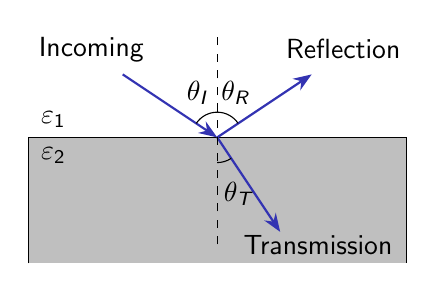
\begin{tikzpicture}[scale=0.8]
    %%Background
    \draw[fill = lightgray] (-3,-2) to (-3,0) to (3,0) to (3,-2);
    %%Wave
    \draw[BlueDefault, thick,-Stealth] (-1.5,1) to (0,0);
    \draw[BlueDefault, thick,-Stealth] (0,0) to (1.5,1);
    \draw[BlueDefault, thick,-Stealth] (0,0) to (1,-1.5);
    \draw
    (-2,1.4) node{Incoming}
    (2,1.4) node{Reflection}
    (1.6,-1.7) node{Transmission}
    ;
    %%Normal plane
    \draw[dashed] (0,-1.7) to (0,1.7);
    %%Angle
    \draw (0,0.4) arc (90:146.3:0.4);
    \draw (0,0.4) arc (90:33.7:0.4);
    \draw (0,-0.4) arc (270:303.7:0.4);
    \draw
    (-0.3,0.7) node{\(\theta_I\)}
    (0.3,0.7) node{\(\theta_R\)}
    (0.35,-0.9) node{\(\theta_T\)}
    ;
    %%Permitivity
    \draw
    (-2.6,0) node[above]{\(\varepsilon_1\)}
    (-2.6,0) node[below]{\(\varepsilon_2\)}
    ;
\end{tikzpicture}

\end{document}